\documentclass[11pt,a4paper]{scrartcl}
\usepackage[utf8]{inputenc}
\usepackage[italian]{babel}

\usepackage{amsmath, amsfonts, amssymb}
\usepackage{graphicx, booktabs}

\usepackage{multirow}
\usepackage{parskip}
\usepackage{pifont}

\newcommand{\yep}{\ding{51}}%
\newcommand{\nope}{\ding{55}}%

\author{L. De Sano, A. Donizetti, M. Scotti}
\title{Risoluzione di sistemi lineari sparsi\\con Python e Scipy}
\date{Maggio 2014}

\begin{document}
\maketitle
\begin{abstract}
Descriviamo l'utilizzo del linguaggio Python e di un ambiente di librerie denominato \emph{Scipy} per la risoluzione di sistemi lineari sparsi.
\end{abstract}

\section*{Python e Scipy}

In questa sezione diamo una descrizione del linguaggio di programmazione (Python) e dell'ambiente di librerie per il calcolo scientifico (Scipy) utilizzati nel progetto. Dettagliamo i criteri che hanno orientato la scelta, e spieghiamo brevemente come e perché Python e Scipy soddisfano effettivamente le nostre aspettative.

\subsection*{Python}

Python\footnote{\texttt{python.org}} è un linguaggio di programmazione \emph{open-source}, \emph{general-purpose} e di alto livello che supporta vari paradigmi di programmazione (tra cui imperativo, ad oggetti, funzionale). È un linguaggio dinamico con una sintassi che facilita la scrittura di codice mantenibile e leggibile, ed è considerato particolarmente adatto per lo sviluppo rapido di applicazioni software e/o di scripting. Poiché tutti e tre i componenti del gruppo avevano esperienza pregressa di programmazione in Python, l'abbiamo immediatamente preso in considerazione.

Le caratteristiche da noi desiderate per l'ambiente con cui effettuare l'esecuzione dei test proposti sui sistemi lineari sparsi sono le seguenti:
\begin{itemize}
	\item \textbf{rapidità di sviluppo}: il linguaggio deve permettere lo sviluppo rapido di codice anche poco strutturato (in totale qualche centinaio di righe di codice che effettuano il setup delle librerie ed eseguono una serie di test);
	\item \textbf{maturità del linguaggio}: il linguaggio deve essere diffuso, ben supportato su varie piattaforme di computazione, semplice da installare e ben documentato;
	\item \textbf{disponibilità di librerie}: il linguaggio deve essere dotato di una libreria per il calcolo scientifico (e in particolar modo per la manipolazione di matrici sparse) ben testata e ben documentata (sia a livello di documentazione primaria, sia per quanto riguarda la disponibilità di materiale esterno come tutorial e discussioni riguardo problemi e modalità d'utilizzo della libreria stessa);
	\item \textbf{performances}: il linguaggio (e le sue librerie) devono fornire gli strumenti adatti ad eseguire computazioni di natura pesantamente numerica in maniera efficiente (ovvero il linguaggio di per sé non deve astrarre troppo dall'architettura hardware del calcolatore, o qualora lo faccia deve fornire un'interfaccia che consenta la chiamata di procedure di basso livello, ad esempio scritte in altri linguaggi di programmazione);
\end{itemize}

Il requisito sulla rapidità di sviluppo è stato il principale motivo per cui abbiamo deciso di escludere in prima battuta l'utilizzo di alcuni dei linguaggi compilati tipicamente usati in ambito computazione scientifica (C, C++, FORTRAN), e di orientarci sulla categoria dei linguaggi dinamici (in genere molto più versatili e adatti all'ambito scripting e software prototyping). 

Per quanto riguarda la maturità dell'ambiente di programmazione, è indubbio che il Python soddisfi il requisito sopracitato: il linguaggio è diffusamente utilizzato, ben documentato, ben supportato e attivamente sviluppato. Decisamente ben pubblicizzata è anche l'esistenza di un ambiente di programmazione adatto alla computazione scientifica (Scipy), su cui ci soffermeremo nella sezione successiva. L'interprete originale (CPython) e le librerie standard sono preinstallati sulla maggior parte dei sistemi Linux e su OS X, ed è disponibile un installer per i sistemi Windows. L'installazione di librerie aggiuntive (distribuite separatamente da quella standard) è lievemente più complicata, soprattutto nel caso di codice che ha anche dipendenze esterne (come nel caso di Scipy).

L'ultimo punto è l'unico che avrebbe potuto rivelarsi problematico: è noto come i linguaggi dinamici (solitamente interpretati, come appunto lo è il Python) tipicamente hanno la peggio nel confronto con i linguaggi compilati in termini di \emph{performances}\footnote{Questo è ancora più evidente per codice dinamico sviluppato rapidamente e senza che la questione performances sia stata considerata accuratamente durante lo fase di progettazione}. Per questo motivo, nella scelta delle librerie esterne da utilizzarsi per la manipolazione di matrici, abbiamo avuto cura di utilizzare un ambiente di programmazione (Scipy, appunto) che non fosse completamente scritto in Python puro, ma che mettesse invece a disposizione un'interfaccia Python per l'utilizzo di librerie \emph{high-performances} scritte in altri linguaggi, e opportunamente racchiuse in \emph{wrappers} Python. Questo ci ha consentito di utilizzare a nostro vantaggio la rapidità di sviluppo fornita da un linguaggio dinamico senza tuttavia dover rinunciare ad ottenere ottime \emph{performaces} sulle computazioni numeriche effettuate durante i test.


\subsection*{Scipy}
Scipy\footnote{\texttt{scipy.org}} è un ecosistema di librerie \emph{open-source} pensate per la scrittura di codice nell'ambito della computazione scientifica. Consiste in una serie di pacchetti (strettamente integrati tra loro) che implementano funzionalità di manipolazione array multidimensionali (Numpy), calcolo numerico ed ottimizzazione (Scipy-library), realizzazione di grafici e schemi (Matplotlib) e computazioni simboliche (Sympy).

Come anticipato nella sezione precedente, per eseguire computazioni numericamente intensive scritte in Python a livelli di \emph{performances} accettabili è necessario delegare la maggior parte delle operazioni di basso livello a librerie specializzate, sviluppate in linguaggi più adatti a tale compito. Scipy non fa eccezione e, pur mantenendo un'interfaccia di alto livello, esegue buona parte delle computazioni numeriche affidandosi a del codice che gira al di fuori dell'interprete Python e scritto in \texttt{C} o in \texttt{FORTRAN}. 

Per quanto riguarda lo stato di salute della libreria, Scipy è attualmente attivamente sviluppato. Come è possibile apprendere da sito ufficiale del progetto, l'ultimo rilascio di Scipy e Numpy è del 3 maggio 2014. Tutto lo sviluppo delle librerie è effettuato su Github, e questo permette una grande flessibilità di sviluppo: centinaia di sviluppatori sottomettono al gruppo di lavoro i propri miglioramenti, e il progetto di cresce rapidamente acquisendo funzionalità sempre nuove. Peraltro, come succede per ogni altro software, e soprattutto per quelli opensource, nelle librerie sono presenti alcuni bug, e alcune funzionalità dei pacchetti sono attualmente prototipate ma non ancora implementate.

La sezione dove sono discusse tematiche relative all'utilizzo del progetto è molto ricca, ed è estremamente facile trovare in rete tutorial scritti da terze parte e risposte ad eventuali problemi incontrati durante lo sviluppo del codice. In caso di segnalazione di bug e/o difetti, la comunity è molto attenta e rapida nel dare una risposta alla questione posta. 

% non ho capito bene che vuol dire:
% --> "Tutte le librerie che compongono l'ambiente Scipy  hanno una milestone molto ricca"  <--
%
% che prevede l'introduzione di sempre nuove funzionalità di analisi e simulazione oltre al miglioramento e alla risoluzione delle problematiche aperte.
%
% TODO: de-commentare il paragrafo una volta chiarita la questione

\subsection*{Scipy per la soluzione di sistemi sparsi}

Per la risoluzione di sistemi lineari sparsi è stato utilizzato il modulo \texttt{scipy.sparse} (per l'importazione e la manipolazione di matrici sparse) e il sottomodulo \texttt{sparse.linalg} (che contiene i risolutori diretti e iterativi specializzati per operare su matrici sparse). Entrambi i moduli utilizzano a loro volta il pacchetto \texttt{numpy}.

Per la manipolazione di matrici, \texttt{numpy} utilizza prevalentemente codice C e chiamate a ATLAS\footnote{Implementazione \emph{open-source} di BLAS} e LAPACK\footnote{Linear Algebra PACKage, scritto in FORTRAN}, mentre il modulo \texttt{scipy.sparse.linalg} utilizza UMFPACK\footnote{Unsymmetric multifrontal sparse LU factorization (\texttt{cise.ufl.edu/research/sparse/umfpack}), scritto in C e chiamato tra l'altro dall'operatore $\setminus$ di Matlab quando le matrici sono sparse} e SuperLU\footnote{Supernodal LU (\texttt{crd-legacy.lbl.gov/$\sim$xiaoye/SuperLU})} per i risolutori diretti. I risolutori iterativi sono implementati in Python puro, ma possono venire precondizionati tramite fattorizzazioni LU parziali calcolate da SuperLU, e risultano quindi in ogni caso abbastanza veloci.

Proprio a causa di queste dipendenze esterne, l'installazione di Scipy è maggiormente soggetta a problemi rispetto a quanto accade solitamente con altre librerie Python. Nonostante l'ambiente Scipy sia ben strutturato a livello di pacchetti e supportato, la modalità di installazione più semplice prevede l'utilizzo almeno di un \emph{package-manager} di sistema (tipicamente presenti su sistemi Linux, vedi aptitude), che si occupa anche di installare e linkare pacchetti esterni (implementazioni BLAS, UMFPACK e altri). La presenza di queste librerie è fondamentale per il funzionamento di Scipy, e non è del tutto banale configurare correttamente il sistema per usarle nel caso si scelga di effettuare un'installazione manuale.

Le dipendenze esterne vanno anche a compromettere leggermente la portabilità del linguaggio: se è quasi garantito che del codice che utilizza solamente la libreria standard sia in grado di girare su sistemi diversi, abbiamo riscontrato invece delle inconsistenze (sulle quali dettaglieremo in seguito) nell'esecuzione su calcolatori differenti di test che utilizzano codice Scipy. 

\section*{Risoluzione di sistemi sparsi}

In questa sezione diamo una descrizione della progettazione, della scrittura e dell'esecuzione dei test proposti. Il lavoro si è svolto sostanzialmente in due fasi: in prima battuta è stato affrontato il problema di leggere le matrici dai files e memorizzare le stesse in RAM in un formato opportuno, successivamente è stato sviluppato il codice che si occupa di chiamare i vari risolutori messi a disposizione da Scipy, misurare tempi di esecuzione ed errori sui risultati, e infine esportare i risultati.

\subsection*{Metodologia di testing}
Il codice Python che implementa i test da noi effettuati è relativamente semplice. In ordine, ciò che viene fatto è
\begin{itemize}
	\item Leggere le matrici dal disco (una sola volta) e immagazzinarle in RAM in un formato opportuno
	\item Calcolare, per ogni matrice $A$, un termine noto $b$ tale che valga $A\overline{x} = b$, con $\overline{x} = (0, 1, 2, \dots)$
	\item Risolvere il sistema lineare $Ax = b$ utilizzando i risolutori diretti e iterativi messi a disposizione da Scipy
	\item Calcolare l'errore commesso come err = $\tfrac{\parallel \overline{x} - x \parallel}{\parallel \overline{x} \parallel}$
	\item Stampare su file tempi di esecuzione ed errori commessi
\end{itemize}

\subsection*{Lettura dei file e memorizzazione}
Date le dimensioni complessive dei files contenenti le matrici (circa 290 MB), una prima questione da affrontare è stata la scelta di una modalità di lettura e costruzione delle strutture dati che sia il più efficiente possibile. In particolare, sarebbe desiderabile ottimizzare i tempi di lettura dal disco, lo spazio occupato dalle matrici in RAM, e i tempi di esecuzione dei metodi per la risoluzione dei sistemi lineari sparsi che esse rappresentano.

\subsubsection*{Lettura da disco}

Per la lettura da disco ci sono (almeno) tre modi di operare:
\begin{itemize}
\item \textbf{Handmade, non bufferizzato}: scrivere uno script Python che legge i dati dal disco, senza bufferizzazione, e costruisce in maniera incrementale le matrici sparse
\item \textbf{Handmade, bufferizzato}: uno script Python che legge i dati dal disco, con bufferizzazione (ovvero lettura di grossi blocchi di dati e costruzione per blocchi)
\item \textbf{mmread}: un metodo messo a disposizione da \texttt{scipy.io} per la lettura di matrici memorizzate in formato Matrix Market\footnote{\texttt{math.nist.gov/MatrixMarket/formats.html\#MMformat}}
\end{itemize}

Il primo (handmade, non bufferizzato) è certamente il più ingenuo. Non è stato realmente preso in considerazione in fase di scrittura del codice, ma ne abbiamo implementato una versione di prova per verificare quanto effettivamente possa costare, in termini di tempi di esecuzione, uno script di importazione dati che sia stato progettato sbadatamente. Il secondo (handmade, bufferizzato) garantisce una buona velocità di lettura e ci ha consentito di utilizzare direttamente i file forniti. Il terzo (\texttt{mmread}) è il più performante, e sicuramente quello che richiede meno lavoro nel caso i file siano formattati secondo lo standard Matrix Market.

Sono riportati (Figura \ref{lettura}) i risultati di tre test di lettura eseguiti sulle sei matrici non simmetriche. Come si può vedere, uno script che sia ben progettato (e che bufferizzi le letture) è equiparabile in velocità di lettura al metodo \texttt{mmread} fornito da \texttt{scipy}, mentre uno non particolarmente ben scritto scala decisamente male rispetto all'aumentare delle dimensioni dei files.

\begin{figure}[!ht]
\centering
\begin{tabular}{l|cc}
\toprule
& time & speed \\
\midrule
nonbuff & 121.56 secs & 1.56 MB/s \\
buff & 27.38 secs & 6.92 MB/s \\
\texttt{mmread} & 12.34 secs & 15.62 MB/s \\
\bottomrule
\end{tabular}
\caption{tempi e velocità di importazione complessivi delle 6 matrici}
\label{tabella1}
\end{figure}

\begin{figure}[!ht]
\centering
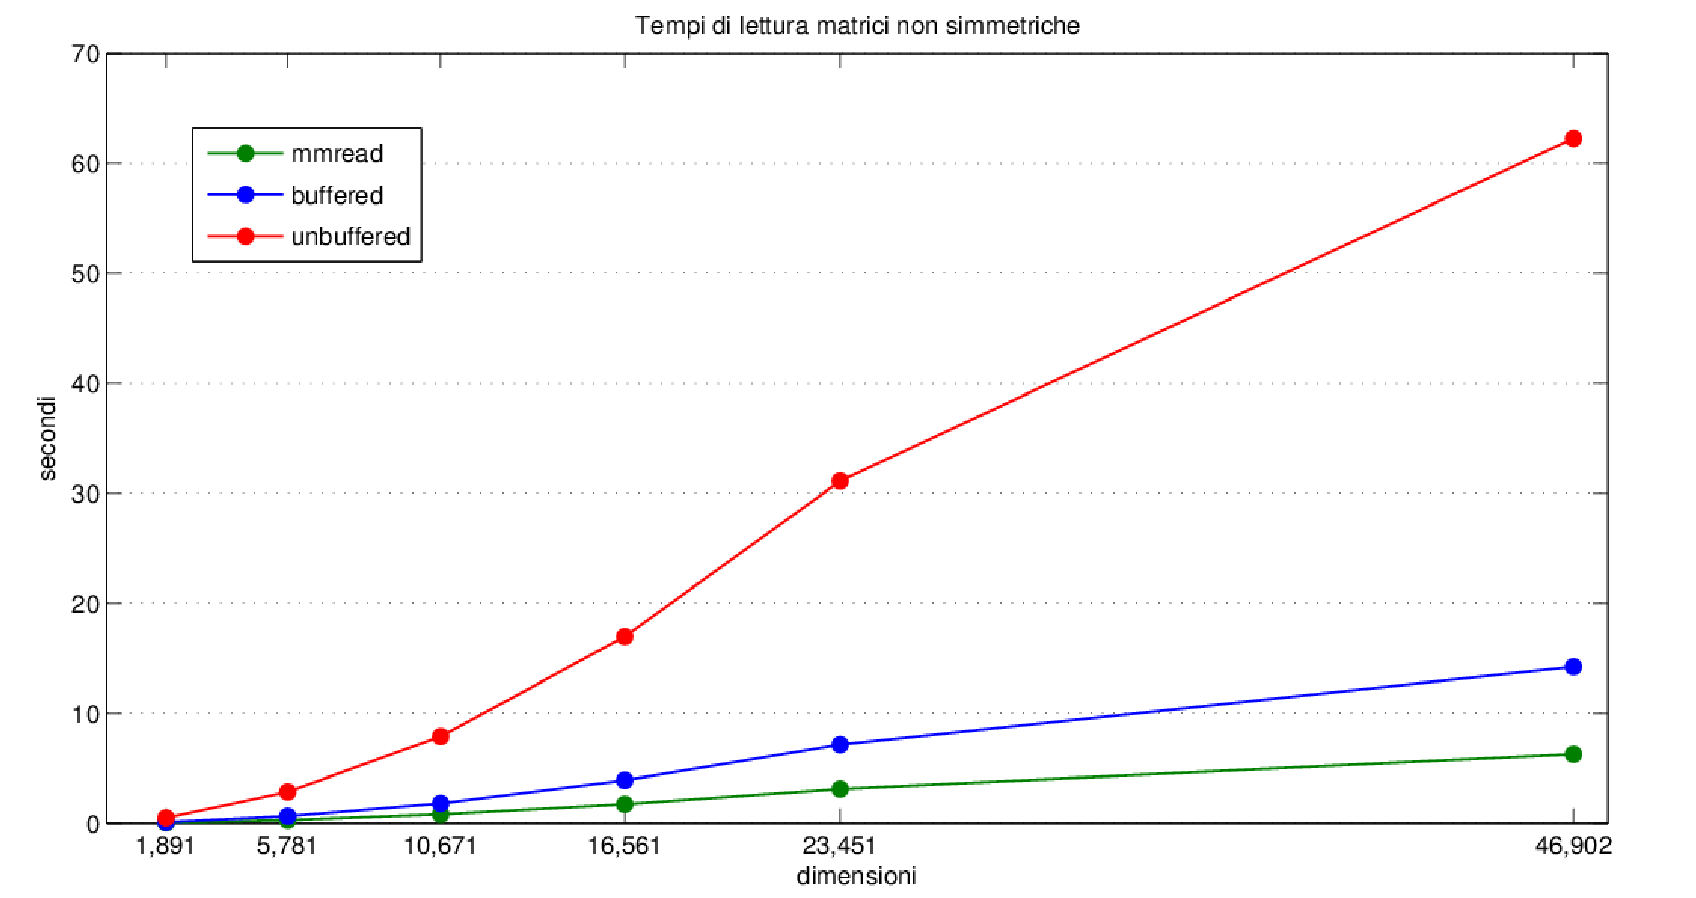
\includegraphics[scale=0.51]{images/lettura} 
\caption{Tempi di lettura per le matrici fornite}
\label{lettura}
\end{figure}

In fase di test dei metodi risolutivi abbiamo infine optato per l'utilizzo di \texttt{mmread} (il più rapido), dopo aver convertito le matrici scaricate nel formato Matrix Market e averne salvato i file.

\subsubsection*{Memorizzazione}

Una volta letti i dati dal disco, è necessario scegliere il formato con cui memorizzare la matrice in RAM. Scipt ne mette a disposizione diversi: \texttt{coo} (coordinate format), \texttt{csc / crs} (compressed sparse columns/rows format), \texttt{dok} (dictionary of keys), e altri. Inizialmente avevamo optato per il formato \texttt{coo} (perché il più semplice su cui mappare il formato dei file di testo contenenti le matrici), ma degli \texttt{SparseEfficiencyWarning} sollevati dall'ambiente durante la risoluzione dei sistemi ci hanno successivamente spinto a convertire le matrici in formato \texttt{csc}, per motivi implementativi il preferito dai risolutori di sistemi integrati in Scipy. Peraltro la conversione si riduce semplicemente alla chiamata di un metodo di casting in fase di importazione.

\subsection*{Metodi diretti}
Il principale metodo diretti messo a disposizione da Scipy per la risoluzione di sistemi lineari sparsi è rappresentato da \texttt{scipy.sparse.linalg.spsolve}. La funzione si tratta in realtà di un wrapper Python attorno a UMFPACK e superLU, e richiede uno sforzo di configurazione minimo. In effetti è sufficiente passare al metodo la matrice sparsa e il vettore dei termini noti, e la funzione si occupa di configurare le librerie C sottostanti in maniera ottimale.

Oltre a \texttt{spsolve}, abbiamo voluto testare anche un procedimento di risoluzione "manuale": una semplice fattorizzazione LU sulla matrice $A$ e successivo calcolo di $x$ operando sulle matrici a scala ottenute (comunque utilizzando le funzioni messe a disposizione da Scipy).

\texttt{spsolve} si è rivelato più veloce del procedimento manuale (probabilmente in virtù di stratagemmi di configurazione nascosti nel wrapper). Non abbiamo invece rilevato alcuna differenza (né sui tempi necessari per la risoluzione dei sistemi, né sugli errori commessi) tra le sei matrici simmetriche definite positive e le sei matrici non simmetriche. 

\subsubsection*{Risultati dei test}

I tempi di risoluzione (Figura \ref{tempi_diretti}) sono del tutto accettabili: pochi millisecondi per le matrici più piccole, e con \texttt{spsolve} sotto i 3 secondi anche nel caso della matrice più grande ($46902 \times 46902$, con oltre 2 milioni di nonzeri). Questo vale sia che per le matrici simmetriche che per le non-simmetriche, e da qui la presenza di un singolo grafico: non abbiamo infatti rilevato che differenze minime (probabilmente dovute a rumore nei test) tra i dati generati dai due tipi di matrici.

\begin{figure}[!ht]
\centering
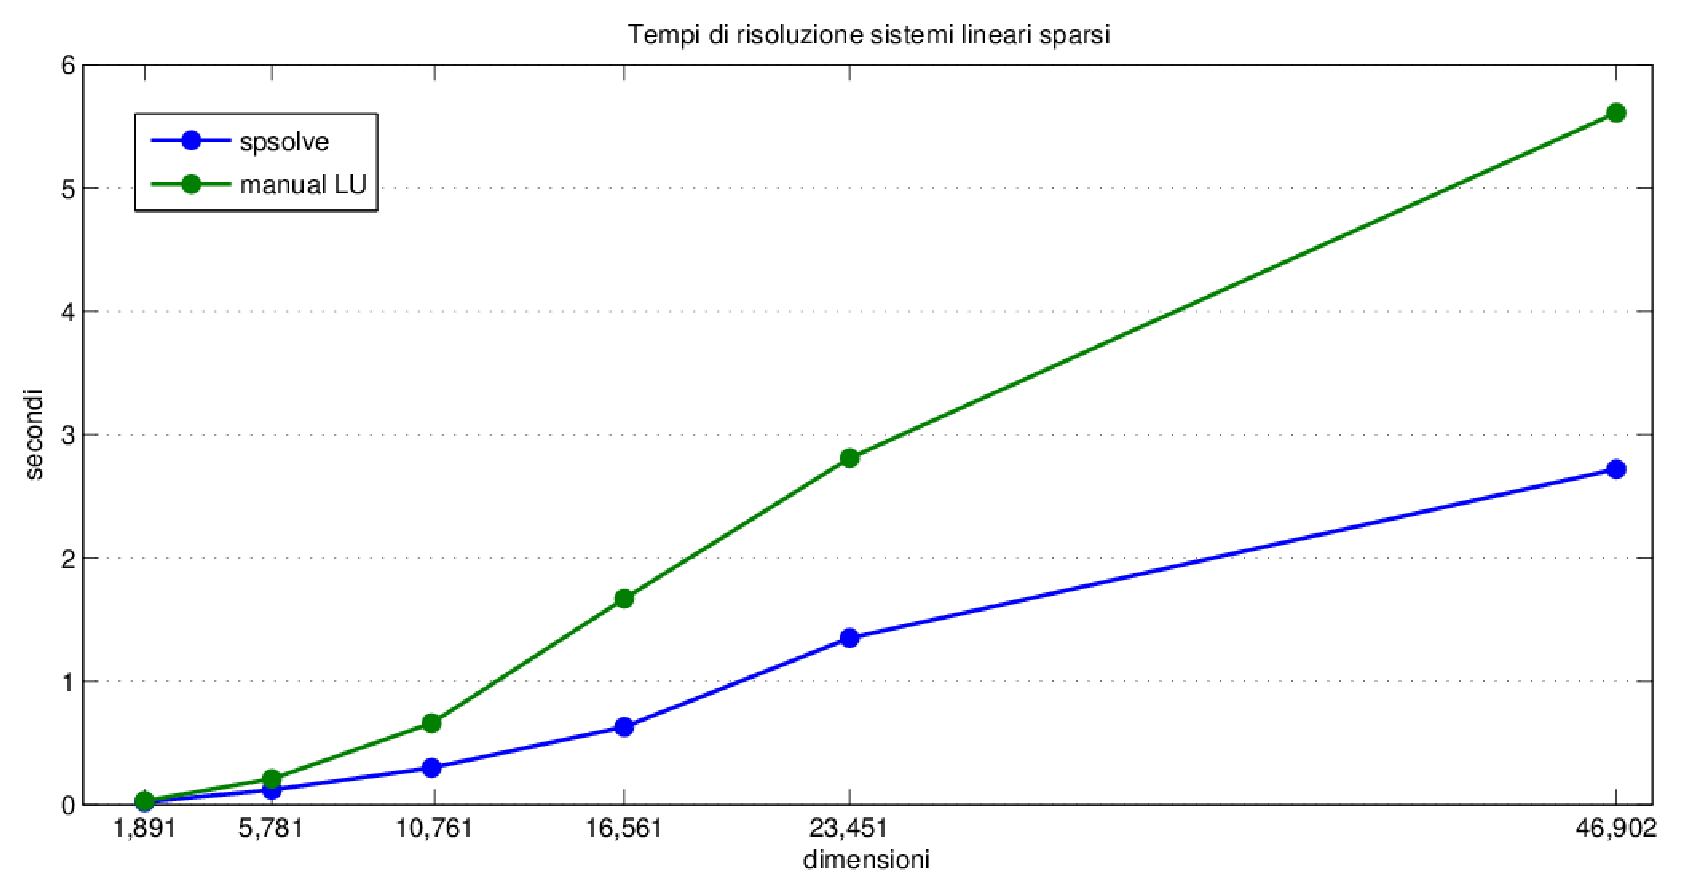
\includegraphics[scale=0.50]{images/tempi_diretti} 
\caption{Tempi di risoluzione con i metodi diretti}
\label{tempi_diretti}
\end{figure}

Gli errori commessi dai metodi diretti (Figura \ref{errori_diretti}) sono vicini alla precisione macchina per le matrici più piccole, mentre sono di diversi ordini di grandezza più grandi per le ultime matrici. In ogni caso entrambi i metodi riescono a mantenere l'errore al di sotto del valore di $10^-6$ richiesto dal testo del progetto. Va comunque fatto notare che \texttt{spsolve} e i metodi per la fattorizzazione LU non mettono a disposizione strumenti per controllare l'errore commesso in fase di risoluzione.

\begin{figure}[!ht]
\centering
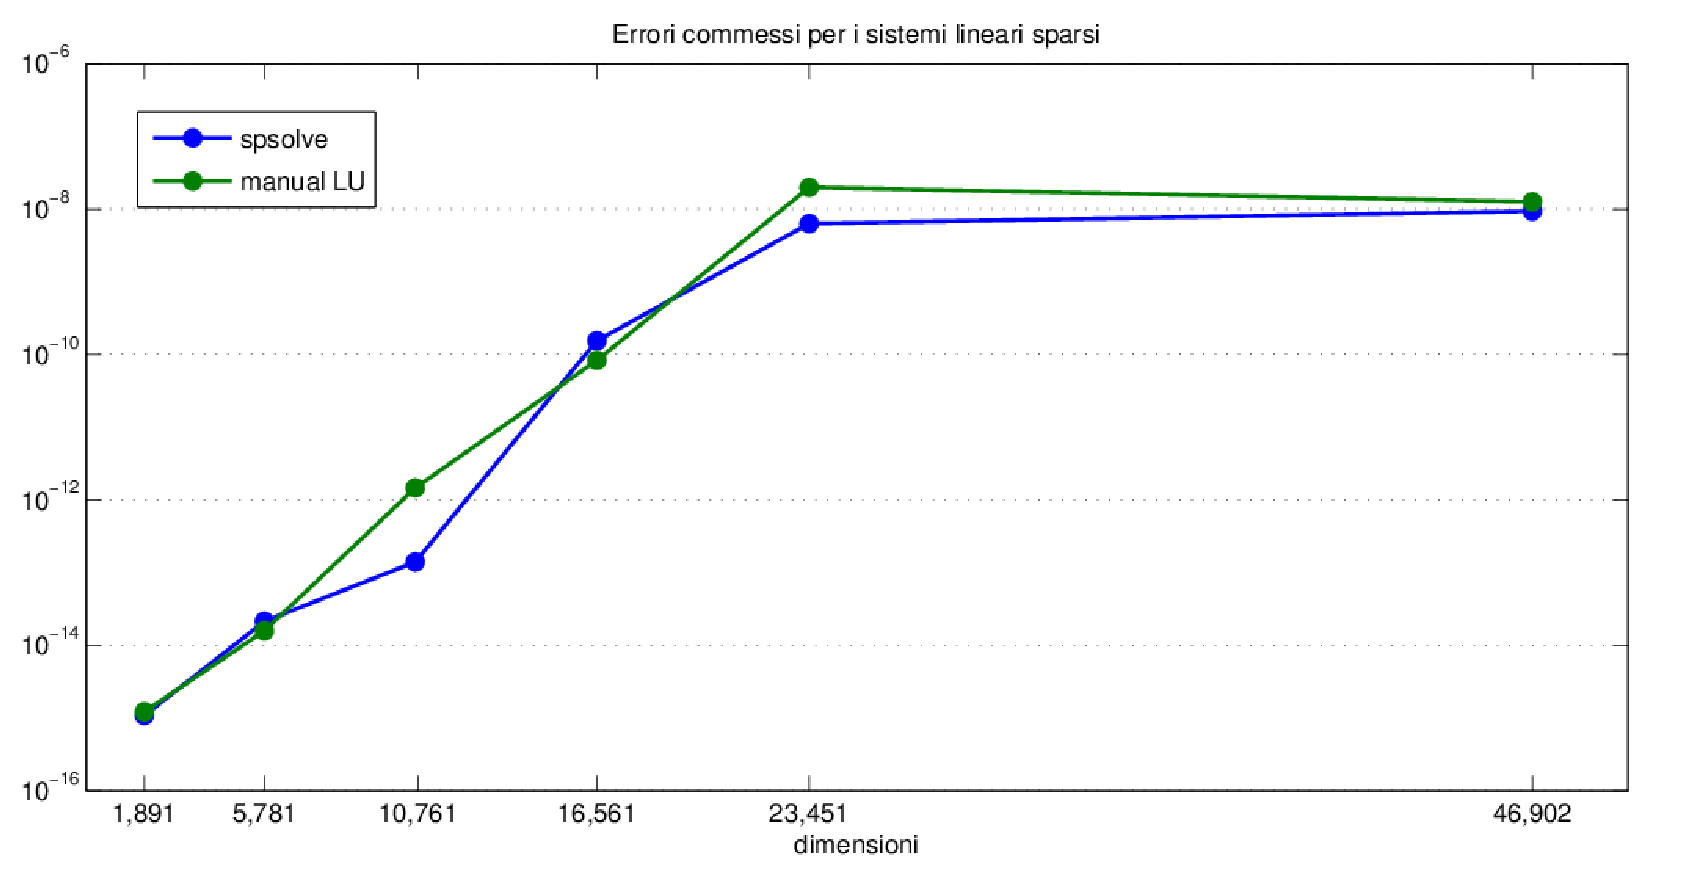
\includegraphics[scale=0.50]{images/errori_diretti} 
\caption{Errori sulla soluzione con i metodi diretti}
\label{errori_diretti}
\end{figure}

\subsection*{Metodi iterativi}
Scipy mette a disposizione parecchi metodi iterativi utilizzabili per la risoluzione di sistemi lineari sparsi. Nei nostri test abbiamo provato ad utilizzare i seguenti:
\begin{itemize}
	\item \texttt{sparse.linalg.bicstab} (BIConjugate Gradient STABilized)
	\item \texttt{sparse.linalg.cg} (Conjugate Gradient)
	\item \texttt{sparse.linalg.cgs} (Conjugate Gradient Squared)
	\item \texttt{sparse.linalg.lgmres} (L. Generalized Minimal RESidual)
	\item \texttt{sparse.linalg.minres} (MINimum RESidual)
\end{itemize}

Nonostante con i metodi sopra elencati sia stato in genere possibile ottenere soluzioni approssimate abbastanza buone in tempi ragionevoli, configurare correttamente i risolutori non è del tutto banale.

\subsubsection*{Tolleranza}

In primo luogo, sebbene tutte le funzioni diano la possibilità di passare un parametro opzionale \texttt{tol}, questo non è utilizzabile per controllare in maniera affidabile l'errore commesso sulla soluzione. Il parametro è documentato come

\begin{quote}
\textbf{tol}: \texttt{float} \\
Tolerance to achieve. The algorithm terminates when either the relative or the absolute residual is below \texttt{tol}.
\end{quote}

La documentazione non fornisce tuttavia alcuna spiegazione riguardo il modo in cui la tolleranza della soluzione corrente viene calcolata, e settare \texttt{tol = 1e-6} porta ad ottenere errori estremamente variabili: sotto $10^{-9}$ per le matrici più piccole, e nell'ordine dei $10^{-1}$ per le matrici più grandi. Errori che peraltro sembrano dipendere fortamente dal metodo iterativo utilizzato: ad esempio a \texttt{bicstab} basta un \texttt{tol = 1e-8} per risolvere tutti i sistemi mantenendo l'errore al di sotto di $10^{-6}$, mentre altri metodi (pur convergenti correttamente!) richiedono di settare \texttt{tol = 1e-15}. Questo comportamento inaspettato sembrerebbe essere dovuto ad un problema nelle routines FORTRAN sottostanti, e in effetti una \emph{issue}\footnote{github.com/scipy/scipy/issues/2694l} che dettaglia sul problema è correntemente aperta su Github (dove è coordinato lo sviluppo di Scipy).

Un primo modo per aggirare il problema consiste nel settare manualmente per ogni metodo le tolleranze, in modo che l'errore sulla matrice più grande sia al di sotto del valore $10^{-6}$, ma questo (oltre a richiedere un certo numero di esperimenti), genera ulteriori problemi. Ad esempio, settando \texttt{tol = 1e-15} con \texttt{cg} porta ad un errore finale dell'ordine di $10^{-7}$ sulla matrice $46902 \times 46902$, ma ad una precisione invece eccessiva sulla matrice più piccola $1891 \times 1891$, andando di fatto a impedire una convergenza rapida.

Il problema è stato infine da noi risolto utilizzando un parametro opzionale messo a disposizione da Scipy: \texttt{callback}. Le funzioni che implementano i metodi iterativi consentono al chiamante di passare una funzione di callback, che viene chiamata al termine di ogni iterazione con parametro \texttt{xk}, la soluzione corrente del sistema. Per ottenere degli errori uniformi sulle matrici di tutte le dimensioni è quindi possibile passare come callback una funzione che controlla se l'errore corrente è sotto il valore $10^{-6}$, e in caso positivo salva il valore di \texttt{xk} e solleva un'eccezione. L'eccezione non può venir catturata al livello della funzione Scipy, che quindi termina l'esecuzione e solleva a sua volta l'eccezione al livello superiore (quello dove c'è il codice dei test). A quel punto l'eccezione viene catturata, e la soluzione ottenuta salvata come soluzione finale della procedura.

\subsubsection*{Precondizionamento}

Tutti i metodi iterativi testati sono stati chiamati passando alla funzione un precondizionatore \texttt{M}. Nei nostri test abbiamo utilizzato come precondizionatore un'approssimazione dell'inversa della matrice $A$, calcolata utililizzando il metodo \texttt{sparse.linalg.spilu} (sparse incomplete LU factorization). 
Data la dimensione delle matrici (e il fatto che i metodi iterativi sono implementati in Python puro) non è possibile infatti risolvere i sistemi proposti con errore ragionevole senza precondizionare le matrici. Nei test effettuati è stato comunque tenuto conto anche del tempo necessario per computare la fattorizzazione LU approssimata, che in Scipy è delegata alla libreria SuperLU che abbiamo menzionata in precedenza.

\subsubsection*{Risultati dei test}

I risultati dei test di convergenza (per le matrici simmetriche e poi per le nonsimmetriche) sono riportati in tabella (Figura \ref{tabella2}). Come si può notare, non ci sono particolari differenze (quantomeno nella capacità di convergere) tra matrici simmetriche definite positive e matrici non simmetriche. Due dei metodi iterativi testati (Conjugate Gradient Squared e L. Generalized Minimal Residual) convergono entro 500 iterazioni con errori inferiori a $10^{-6}$ sulle matrici di tutte le dimensioni. Conjugate Gradient e Minimum Residual non convergono, rispettivamente, sulle ultime due matrici e sulle ultime tre. L'unica differenza di rilievo tra le due tipologie di matrici la evidenzia Biconjugate Gradient Stabilized, che converge sulla matrice nonsimmetrica più grande ma non sulla simmetrica più grande.

\begin{figure}[!ht]
\centering
\begin{tabular}{cr|ccccc}
\toprule
tipo & dim & \verb|bicgstab| & \verb|  cg   | & \verb|  cgs  | & \verb| lgmres| & \verb| minres| \\
\midrule
\multirow{5}{*}{$\ddots$} & {1891} & \yep & \yep & \yep & \yep & \yep \\
& {5781} & \yep & \yep & \yep & \yep & \yep \\
& {10671} & \yep & \yep & \yep & \yep & \yep \\
& {16561} & \yep & \yep  & \yep & \yep & \nope \\
& {23451} & \yep & \nope & \yep & \yep & \nope \\
& {46902} & \nope & \nope & \yep & \yep & \nope \\ 
\midrule
\multirow{5}{*}{$\square$} & {1891} & \yep & \yep & \yep & \yep & \yep \\
& {5781} & \yep & \yep & \yep & \yep & \yep \\
& {10671} & \yep & \yep & \yep & \yep & \yep \\
& {16561} & \yep & \yep  & \yep & \yep & \nope \\
& {23451} & \yep & \nope & \yep & \yep & \nope \\
& {46902} & \yep & \nope & \yep & \yep & \nope \\ 
\bottomrule
\end{tabular}
\caption{errore sotto $10^{-6}$ (entro 500 iterazioni)}
\label{tabella2}
\end{figure}

I tempi di esecuzione sono graficati in Figura \ref{tempi_iterativi}. \texttt{cgs}, che converge senza particolari problemi sui sistemi di tutte le dimensioni, non impiega più di 10 secondi per terminare la computazione sulla matrice più grande. Anche i metodi che non convergono entro le 500 iterazioni sulle ultime matrici sono in grado di risolvere i sistemi lineari più piccoli, peraltro in tempi assai vicini a quelli impiegati dagli altri metodi. Questo è probabilmente dovuto al fatto che sulle prime matrici i tempi di esecuzione sono dominati dal tempo di calcolo del precondizionatore (LU approssimata, uguale per tutti i metodi da noi testati). Man mano che le dimensioni del problema aumentano, il fattore dominante diventa il tempo impiegato nelle iterazioni, e solo i metodi più performanti si dimostrano in grado di convergere in tempi brevi. 

\begin{figure}[!ht]
\centering
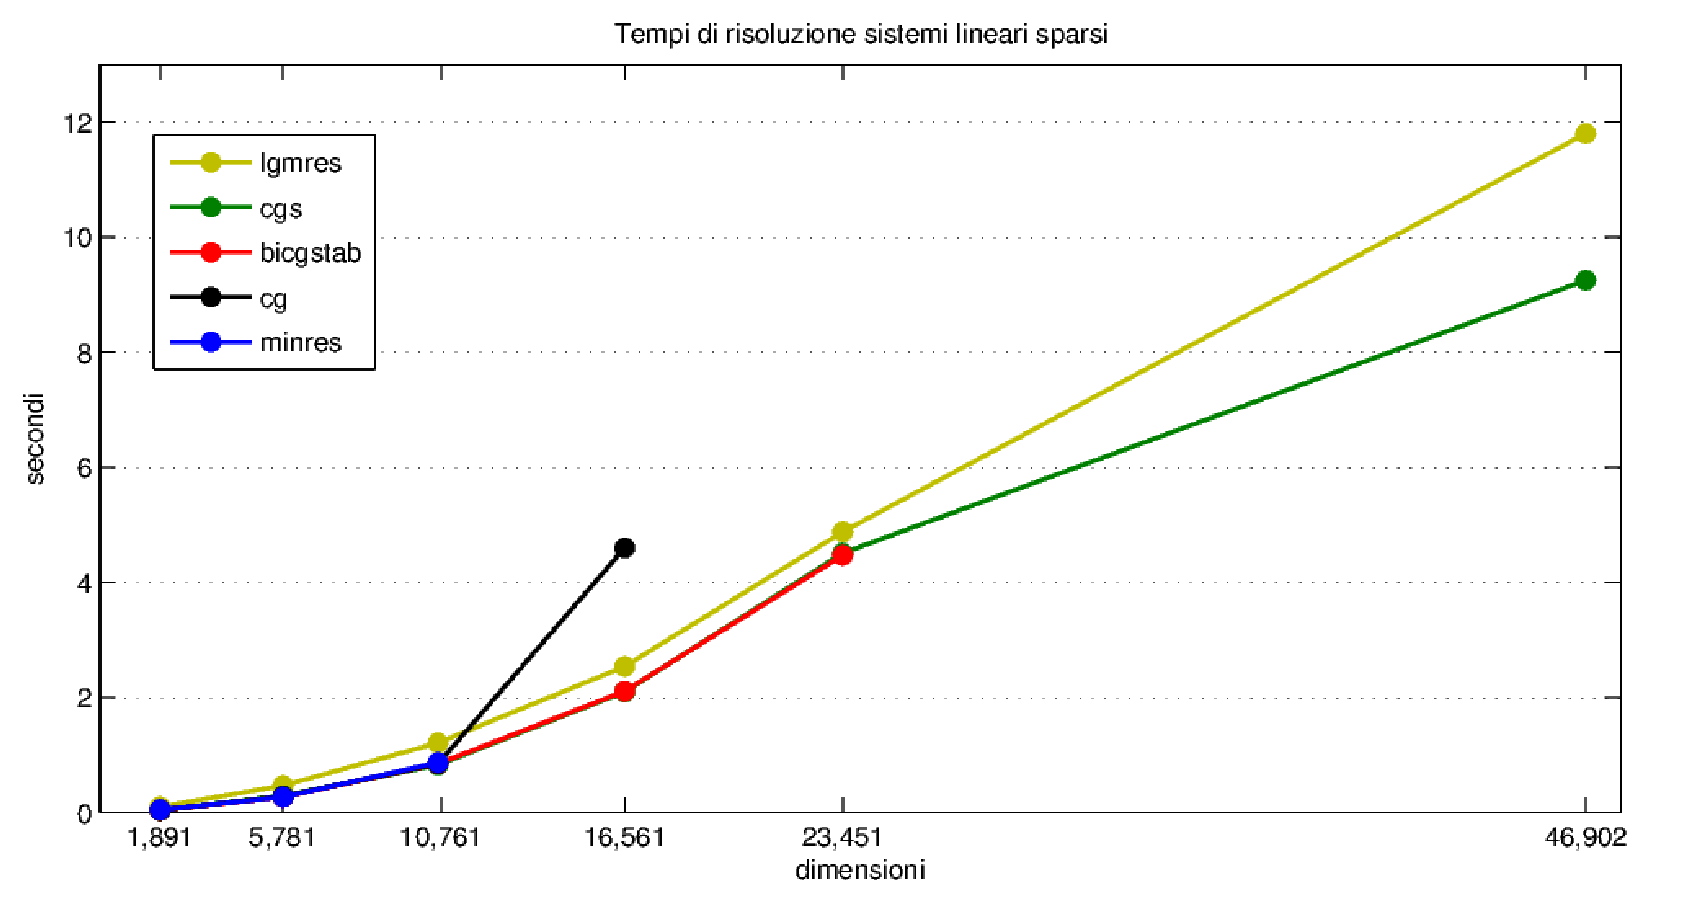
\includegraphics[scale=0.51]{images/tempi_iterativi} 
\caption{Tempi di risoluzione (simmetriche) con i metodi iterativi}
\label{tempi_iterativi}
\end{figure}

Non riportiamo il grafico dei tempi necessari per la soluzione dei sistemi derivati dalle matrici nonsimmetriche perché i valori ottenuti dai test si discostano di pochissimo (meno del 5\%) da quelli rilevati per le matrici simmetriche definite positive. Rileviamo quindi che i metodi iterativi messi a disposizione da Scipy non sembrano discriminare tra le due tipologie di matrici coinvolte nei test (quantomeno per matrici delle dimensioni da noi testate). Sia i tempi necessari alla convergenza che la capacità stessa di convergere sono del tutto analoghi, per i vari metodi, tra matrici aventi le stesse dimensioni.

Riportiamo anche, al fine di fare un confronto complessivo tra i metodi testati, un grafico che contiene i dati relativi ai tempi di risoluzione e agli errori commessi sulla matrice nonsimmetrica più grande (per i metodi che hanno restituito una soluzione corretta). Quel che si nota è che per matrici sparse di dimensioni vicine a 50000$\times$50000 e con una percentuale di nonzeri intorno allo $0.1\%$, i due metodi diretti (\texttt{spsolve} e la scomposizione LU) sono i più rapidi a fornire una soluzione entro $10^{-6}$ da quella esatta. I metodi iterativi, pur riuscendo a convergere in tempi relativamente rapidi, non sembrano essere  competivi su matrici sparse aventi le dimensioni di quelle da noi testate.

\begin{figure}[!ht]
\centering
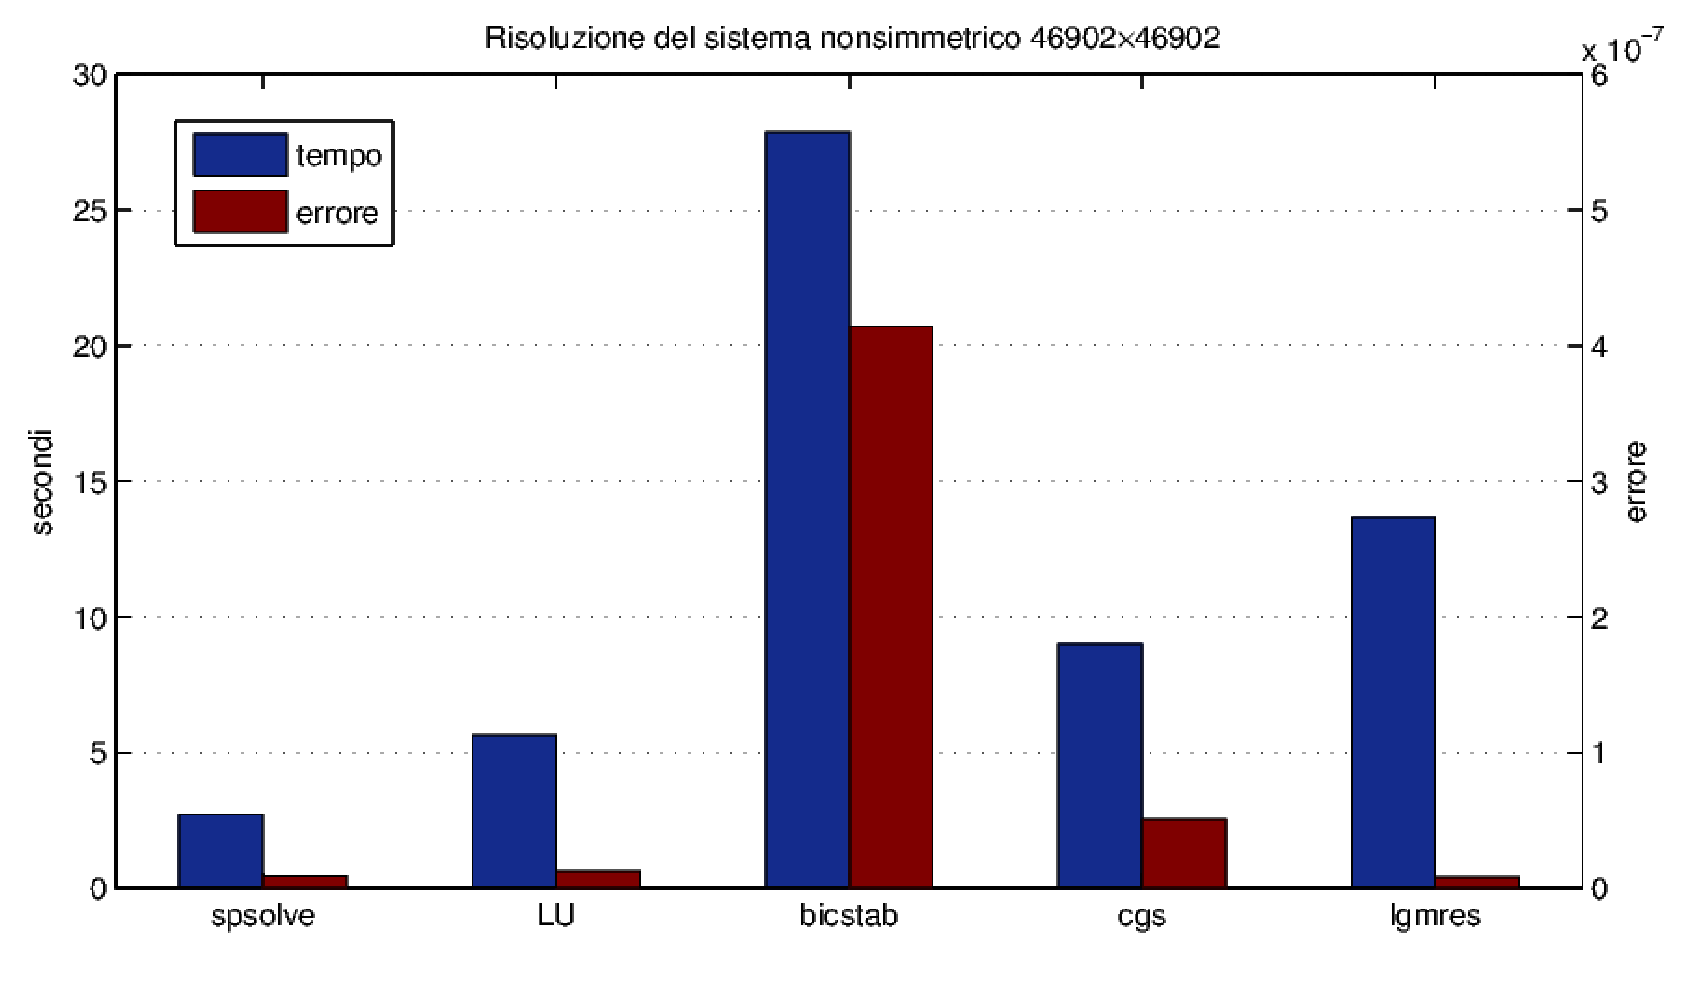
\includegraphics[scale=0.50]{images/confronto} 
\caption{Tempi ed errori sul sistema 46902$\times$46902}
\label{confronto}
\end{figure}

\newpage
\subsection*{Problematiche incontrate}
Abbiamo già citato, nel corso della discussione, alcune delle problematiche incontrate durante lo sviluppo e l'esecuzione dei nostri test. Ne riportiamo in questa sezione un elenco esaustivo.

\begin{itemize}
\item non è chiarito in che modo il parametro opzionale \texttt{tol} venga gestito dai metodi iterativi per l'arresto della procedura risolutiva. (\textsf{difetto nella documentazione})
\item settare manualmente \texttt{tol} porta a risultati poco consistenti. Uno stesso valore (es. \texttt{tol = 1e-8}) può bastare per la convergenza su alcune matrici, e con alcuni metodi, e non bastare su altre matrici, o con altri metodi. (\textsf{probabile BUG delle routines sottostanti})
\item il metodo \texttt{sparse.linalg.spilu}, usato per le fattorizzazioni LU parziali, è documentato in una maniera che non rende del tutto chiaro quale sia il modo corretto di passare alla funzione alcuni parametri opzionali. (\textsf{difetto nella documentazione})
\item su uno dei sistemi (OS Linux) da noi utilizzati per i test, la chiamata al metodo \texttt{sparse.linalg.spilu} fallisce terminando l'esecuzione con un \texttt{"ERR: Matrix is singular"} sulla matrice simmetrica $10671\times10671$, nonostante la matrice non sia singolare e l'esecuzione dello stesso codice vada a buon fine su uno altro sistema Linux avente \emph{la stessa versione di Scipy} installata. (\textsf{probabile BUG dovuto a differenze tra le librerie C e FORTRAN installate sui due sistemi})
\item alcuni parametri opzionali listati della documentazione non sono effettivamente implementati, e generano  un \texttt{NotImplementedError} quando vengono utilizzati. (\textsf{difetto nella documentazione})
\item nonostante il parametro opzionale \texttt{M} (precondizionatore) sia documentato, e la documentazione di \texttt{spilu} menzioni brevemente il fatto che sia possibile utilizzare il suddetto metodo per precondizionare i sistemi lineari, non è chiaro come possa essere effettivamente implementato il precondizionamento. Infine il metodo migliore si è rivelato essere costruire un \texttt{LinearOperator} a partire della fattorizzazione LU approssimata e passarlo (via puntatore a funzione) ai metodi iterativi testati, metodo tuttavia scoperto per caso in un esempio di codice riportato in una mailing list non associata al progetto Scipy (\textsf{difetto nella documentazione})
\item la documentazione del metodo \texttt{bicgstab} riporta
\begin{quote}
The real or complex N-by-N matrix of the linear system A must represent a hermitian, positive definite matrix
\end{quote}
ma il metodo risolve correttamente sistemi lineari aventi matrice associata asimmetrica. Non è chiaro il motivo della limitazione citata dalla documentazione. La documentazione del metodo Matlab analogo non riporta restrizioni sul formato della matrice. (\textsf{difetto nella documentazione})
\end{itemize}

\subsection*{Conclusione}
L'ecosistema di librerie fornite da Scipy è facilmente utilizzabile per la risoluzione di sistemi lineari sparsi. L'efficienza dei metodi forniti è garantita dall'uso di librerie esterne (C e FORTRAN) per le computazioni numericamente intensive, anche se queste vanno ad impattare sulla portabilità del codice e sulla replicabilità dei risultati ottenuti. L'installazione dell'ambiente Scipy è relativamente più complicata dell'installazione del tipico pacchetto Python, e la gestione delle dipendenze esterne (le librerie numeriche di basso livello) non del tutto triviale. La documentazione pubblicata è molto buona, anche se da sola non sufficiente a fornire tutte le informazioni di cui un utilizzatore occasionale del pacchetto può avere bisogno per la risoluzione di sistemi lineari sparsi. In alcuni casi è di fatto necessario affidarsi a tutorial esterni, peraltro facilmente reperibili tramite motore di ricerca. A giudicare dalla mole di discussioni (tutorials, guide e note di approfondimento fornite da terze parti, domande relative all'utilizzo della libreria, ecc\dots) presenti in rete, il progetto sembrerebbe essere diffusamente utilizzato. L'attività delle mailing lists ufficiali e della pagina Github su cui avviene il lavoro indicano inoltre che il progetto è correntemente attivamente sviluppato.

\end{document}